% Options for packages loaded elsewhere
% Options for packages loaded elsewhere
\PassOptionsToPackage{unicode}{hyperref}
\PassOptionsToPackage{hyphens}{url}
\PassOptionsToPackage{dvipsnames,svgnames,x11names}{xcolor}
%
\documentclass[
]{agujournal2019}
\usepackage{xcolor}
\usepackage{amsmath,amssymb}
\setcounter{secnumdepth}{5}
\usepackage{iftex}
\ifPDFTeX
  \usepackage[T1]{fontenc}
  \usepackage[utf8]{inputenc}
  \usepackage{textcomp} % provide euro and other symbols
\else % if luatex or xetex
  \usepackage{unicode-math} % this also loads fontspec
  \defaultfontfeatures{Scale=MatchLowercase}
  \defaultfontfeatures[\rmfamily]{Ligatures=TeX,Scale=1}
\fi
\usepackage{lmodern}
\ifPDFTeX\else
  % xetex/luatex font selection
\fi
% Use upquote if available, for straight quotes in verbatim environments
\IfFileExists{upquote.sty}{\usepackage{upquote}}{}
\IfFileExists{microtype.sty}{% use microtype if available
  \usepackage[]{microtype}
  \UseMicrotypeSet[protrusion]{basicmath} % disable protrusion for tt fonts
}{}
\makeatletter
\@ifundefined{KOMAClassName}{% if non-KOMA class
  \IfFileExists{parskip.sty}{%
    \usepackage{parskip}
  }{% else
    \setlength{\parindent}{0pt}
    \setlength{\parskip}{6pt plus 2pt minus 1pt}}
}{% if KOMA class
  \KOMAoptions{parskip=half}}
\makeatother
% Make \paragraph and \subparagraph free-standing
\makeatletter
\ifx\paragraph\undefined\else
  \let\oldparagraph\paragraph
  \renewcommand{\paragraph}{
    \@ifstar
      \xxxParagraphStar
      \xxxParagraphNoStar
  }
  \newcommand{\xxxParagraphStar}[1]{\oldparagraph*{#1}\mbox{}}
  \newcommand{\xxxParagraphNoStar}[1]{\oldparagraph{#1}\mbox{}}
\fi
\ifx\subparagraph\undefined\else
  \let\oldsubparagraph\subparagraph
  \renewcommand{\subparagraph}{
    \@ifstar
      \xxxSubParagraphStar
      \xxxSubParagraphNoStar
  }
  \newcommand{\xxxSubParagraphStar}[1]{\oldsubparagraph*{#1}\mbox{}}
  \newcommand{\xxxSubParagraphNoStar}[1]{\oldsubparagraph{#1}\mbox{}}
\fi
\makeatother


\usepackage{longtable,booktabs,array}
\newcounter{none} % for unnumbered tables
\usepackage{calc} % for calculating minipage widths
% Correct order of tables after \paragraph or \subparagraph
\usepackage{etoolbox}
\makeatletter
\patchcmd\longtable{\par}{\if@noskipsec\mbox{}\fi\par}{}{}
\makeatother
% Allow footnotes in longtable head/foot
\IfFileExists{footnotehyper.sty}{\usepackage{footnotehyper}}{\usepackage{footnote}}
\makesavenoteenv{longtable}
\usepackage{graphicx}
\makeatletter
\newsavebox\pandoc@box
\newcommand*\pandocbounded[1]{% scales image to fit in text height/width
  \sbox\pandoc@box{#1}%
  \Gscale@div\@tempa{\textheight}{\dimexpr\ht\pandoc@box+\dp\pandoc@box\relax}%
  \Gscale@div\@tempb{\linewidth}{\wd\pandoc@box}%
  \ifdim\@tempb\p@<\@tempa\p@\let\@tempa\@tempb\fi% select the smaller of both
  \ifdim\@tempa\p@<\p@\scalebox{\@tempa}{\usebox\pandoc@box}%
  \else\usebox{\pandoc@box}%
  \fi%
}
% Set default figure placement to htbp
\def\fps@figure{htbp}
\makeatother





\setlength{\emergencystretch}{3em} % prevent overfull lines

\providecommand{\tightlist}{%
  \setlength{\itemsep}{0pt}\setlength{\parskip}{0pt}}



 


\usepackage{url} %this package should fix any errors with URLs in refs.
\usepackage{lineno}
\usepackage[inline]{trackchanges} %for better track changes. finalnew option will compile document with changes incorporated.
\usepackage{soul}
\linenumbers
\makeatletter
\@ifpackageloaded{caption}{}{\usepackage{caption}}
\AtBeginDocument{%
\ifdefined\contentsname
  \renewcommand*\contentsname{Table of contents}
\else
  \newcommand\contentsname{Table of contents}
\fi
\ifdefined\listfigurename
  \renewcommand*\listfigurename{List of Figures}
\else
  \newcommand\listfigurename{List of Figures}
\fi
\ifdefined\listtablename
  \renewcommand*\listtablename{List of Tables}
\else
  \newcommand\listtablename{List of Tables}
\fi
\ifdefined\figurename
  \renewcommand*\figurename{Figure}
\else
  \newcommand\figurename{Figure}
\fi
\ifdefined\tablename
  \renewcommand*\tablename{Table}
\else
  \newcommand\tablename{Table}
\fi
}
\@ifpackageloaded{float}{}{\usepackage{float}}
\floatstyle{ruled}
\@ifundefined{c@chapter}{\newfloat{codelisting}{h}{lop}}{\newfloat{codelisting}{h}{lop}[chapter]}
\floatname{codelisting}{Listing}
\newcommand*\listoflistings{\listof{codelisting}{List of Listings}}
\makeatother
\makeatletter
\makeatother
\makeatletter
\@ifpackageloaded{caption}{}{\usepackage{caption}}
\@ifpackageloaded{subcaption}{}{\usepackage{subcaption}}
\makeatother
\usepackage{bookmark}
\IfFileExists{xurl.sty}{\usepackage{xurl}}{} % add URL line breaks if available
\urlstyle{same}
\hypersetup{
  pdftitle={Desapariciones en México},
  pdfauthor={José Rubén Alfaro González; Daniela Sanluis},
  colorlinks=true,
  linkcolor={blue},
  filecolor={Maroon},
  citecolor={Blue},
  urlcolor={Blue},
  pdfcreator={LaTeX via pandoc}}


\journalname{Earth and Space Science}

\draftfalse

\begin{document}
\title{Desapariciones en México}

\authors{José Rubén Alfaro González\affil{1}, Daniela Sanluis\affil{1}}
\affiliation{1}{UNAM, }
\correspondingauthor{José Rubén Alfaro González}{rou@ciencias.unam.mx}


\begin{abstract}
Este trabajo analiza el Registro Nacional de Personas Desaparecidas y No
Localizadas de México, publicado por el Secretariado Ejecutivo del
Sistema Nacional de Seguridad Pública (SESNSP). El dataset cuenta con
133,886 registros y 11 variables que incluyen información demográfica,
geográfica y temporal de cada caso. Se identificó que una proporción
considerable de los datos se encuentra marcada como CONFIDENCIAL (hasta
\textasciitilde40\% en algunas columnas) o presenta valores nulos (hasta
\textasciitilde60\% en fechas de nacimiento), lo que motivó la creación
de un sub-dataset limpio para el análisis estadístico. Se calcularon
medidas de localización, variabilidad, heterogeneidad y concentración
sobre variables como edad al momento de la desaparición, sexo, entidad,
municipio, estatus de la víctima y fecha de desaparición. Los resultados
muestran que las desapariciones afectan predominantemente a hombres en
el rango de 17 a 45 años, se distribuyen a lo largo de todo el
territorio nacional, y presentan una tendencia creciente a lo largo del
tiempo.
\end{abstract}

\section*{Plain Language Summary}
Analizamos el registro nacional de personas desaparecidas en México con
más de 133 mil casos. Encontramos que la mayoría de las personas
desaparecidas son hombres de entre 17 y 45 años, y que las
desapariciones ocurren en todos los estados del país, aunque con mayor
concentración en ciertos municipios. La tendencia de desapariciones ha
aumentado con el tiempo, con los años más recientes registrando el mayor
número de casos. Una parte importante de la información está marcada
como confidencial, lo que limita el análisis pero también sugiere que
muchos casos aún están activos o en investigación.




\section{Inicio del análisis}\label{inicio-del-anuxe1lisis}

\subsection{Carga del dataset}\label{carga-del-dataset}

Cargamos el dataset. Además, podemos ver la forma del DS, que contiene
133,886 filas, y 11 columnas. Más información respecto a la información
que proporciona cada una de las columnas será dada en el pdf que
adjuntamos.

\textsubscript{Source:
\href{https://Rou-uu.github.io/pruebaQuarto/index.qmd.html}{Article
Notebook}}

\begin{verbatim}
Dataset cargado exitosamente
Número de filas: 133887
Número de columnas: 11
Primera inspección: 
\end{verbatim}

{\def\LTcaptype{none} % do not increment counter
\begin{longtable}[]{@{}llllllllllll@{}}
\toprule\noalign{}
& ID\_VICTIMA & ORIGEN\_REPORTE & FECHA\_NACIMIENTO & SEXO &
FECHA\_DESAPARICION & FECHA\_REGISTRO & ESTATUS\_VICTIMA & CVE\_ENT &
ENTIDAD & CVE\_MUN & MUNICIPIO \\
\midrule\noalign{}
\endhead
\bottomrule\noalign{}
\endlastfoot
0 & D49C001E-41E4-45B7-B8FD-D867578F093E & FISCALIA GENERAL DE DURANGO &
CONFIDENCIAL & CONFIDENCIAL & CONFIDENCIAL & CONFIDENCIAL & CONFIDENCIAL
& 10 & DURANGO & 999 & CONFIDENCIAL \\
1 & 2D2B5CD4-7AF7-48C3-887E-72F4C6403863 & COMISION LOCAL DE BUSQUEDA DE
PERSONAS DEL EST... & 1971-06-13 & HOMBRE & 2025-09-28 04:40:00 &
2025-09-29 10:00:00 & DESAPARECIDA & 25 & SINALOA & 4 & CONCORDIA \\
2 & 6AE9098C-0C30-4709-9A2C-37F6312CD43E & PROCURADURIA GENERAL DE
JUSTICIA DE LA CIUDAD ... & CONFIDENCIAL & CONFIDENCIAL & CONFIDENCIAL &
CONFIDENCIAL & CONFIDENCIAL & 9 & CIUDAD DE MÉXICO & 999 &
CONFIDENCIAL \\
3 & 6B899D2D-F33D-4880-82CD-953FF972B9C3 & FISCALIA GENERAL DEL ESTADO
BAJA CALIFORNIA & CONFIDENCIAL & CONFIDENCIAL & CONFIDENCIAL &
CONFIDENCIAL & CONFIDENCIAL & 2 & BAJA CALIFORNIA & 999 &
CONFIDENCIAL \\
4 & 3F026638-8169-4CEA-9D9A-E345B6D2D7B6 & FISCALIA GENERAL DEL ESTADO
BAJA CALIFORNIA & CONFIDENCIAL & CONFIDENCIAL & CONFIDENCIAL &
CONFIDENCIAL & CONFIDENCIAL & 2 & BAJA CALIFORNIA & 999 &
CONFIDENCIAL \\
\end{longtable}
}

\textsubscript{Source:
\href{https://Rou-uu.github.io/pruebaQuarto/index.qmd.html}{Article
Notebook}}

También podemos ver los tipos de datos con los que vamos a contar. La
mayoría serán datos categoricos o temporales, pero a partir de estos
podemos calcular ciertos datos que nos serán de utilidad como la edad al
momento de la desaparición (lo haremos más adelante).

\textsubscript{Source:
\href{https://Rou-uu.github.io/pruebaQuarto/index.qmd.html}{Article
Notebook}}

\begin{verbatim}
<class 'pandas.DataFrame'>
RangeIndex: 133887 entries, 0 to 133886
Data columns (total 11 columns):
 #   Column              Non-Null Count   Dtype
---  ------              --------------   -----
 0   ID_VICTIMA          133887 non-null  str  
 1   ORIGEN_REPORTE      133887 non-null  str  
 2   FECHA_NACIMIENTO    105000 non-null  str  
 3   SEXO                133887 non-null  str  
 4   FECHA_DESAPARICION  125727 non-null  str  
 5   FECHA_REGISTRO      127790 non-null  str  
 6   ESTATUS_VICTIMA     133887 non-null  str  
 7   CVE_ENT             133887 non-null  int64
 8   ENTIDAD             133887 non-null  str  
 9   CVE_MUN             133887 non-null  int64
 10  MUNICIPIO           133887 non-null  str  
dtypes: int64(2), str(9)
memory usage: 11.2 MB
\end{verbatim}

\textsubscript{Source:
\href{https://Rou-uu.github.io/pruebaQuarto/index.qmd.html}{Article
Notebook}}

Y la cantidad de valores únicos de cada columna. Hay que tomar en cuenta
que uno de esos valores es CONFIDENCIAL, lo que nos indica que no se
tiene información de esa persona.

\textsubscript{Source:
\href{https://Rou-uu.github.io/pruebaQuarto/index.qmd.html}{Article
Notebook}}

\begin{longtable}[]{@{}lll@{}}
\caption{Valores únicos por columna}\label{T_16ec0}\tabularnewline
\toprule\noalign{}
~ & Columna & Valores\_Unicos \\
\midrule\noalign{}
\endfirsthead
\toprule\noalign{}
~ & Columna & Valores\_Unicos \\
\midrule\noalign{}
\endhead
\bottomrule\noalign{}
\endlastfoot
0 & ID\_VICTIMA & 133,887 \\
5 & FECHA\_REGISTRO & 53,635 \\
4 & FECHA\_DESAPARICION & 50,383 \\
2 & FECHA\_NACIMIENTO & 20,808 \\
10 & MUNICIPIO & 1,554 \\
9 & CVE\_MUN & 275 \\
1 & ORIGEN\_REPORTE & 74 \\
7 & CVE\_ENT & 33 \\
8 & ENTIDAD & 33 \\
3 & SEXO & 4 \\
6 & ESTATUS\_VICTIMA & 3 \\
\end{longtable}

\textsubscript{Source:
\href{https://Rou-uu.github.io/pruebaQuarto/index.qmd.html}{Article
Notebook}}

\subsection{Análisis de datos faltantes y
confidenciales}\label{anuxe1lisis-de-datos-faltantes-y-confidenciales}

A continuación se muestra la cantidad de datos nulos del dataset.
Podemos ver que la mayoría de datos nulos son de los campos de fechas,
ya sea de nacimiento, desaparicion, o de registro. Además, es un
porcentaje bastante alto de información perdida, llegando casi a un 60\%
para fechas de nacimiento, y 43\% para las demás fechas. Fuera de eso,
las demás columnas no tienen datos faltantes, pero falta revisar la
cantidad de datos confidenciales.

También se muestra la cantidad de información confidencial. Se puede ver
que la cantidad de información confidencial en cada columna es la misma,
por lo que podemos intuir que son casos que siguen siendo confidenciales
debido a varias razones (casos abiertos, en proceso de investigación,
etc.)

\textsubscript{Source:
\href{https://Rou-uu.github.io/pruebaQuarto/index.qmd.html}{Article
Notebook}}

\begin{verbatim}
Valores nulos por columna:
           Columna  Valores_Nulos  Porcentaje
  FECHA_NACIMIENTO          28887   21.575657
FECHA_DESAPARICION           8160    6.094692
    FECHA_REGISTRO           6097    4.553840
        ID_VICTIMA              0    0.000000
    ORIGEN_REPORTE              0    0.000000
              SEXO              0    0.000000
   ESTATUS_VICTIMA              0    0.000000
           CVE_ENT              0    0.000000
           ENTIDAD              0    0.000000
           CVE_MUN              0    0.000000
         MUNICIPIO              0    0.000000

Valores confidenciales por columna:
           Columna  Valores_Confidenciales  Porcentaje
  FECHA_NACIMIENTO                   49149   36.709315
              SEXO                   49149   36.709315
FECHA_DESAPARICION                   49149   36.709315
    FECHA_REGISTRO                   49149   36.709315
   ESTATUS_VICTIMA                   49149   36.709315
         MUNICIPIO                   49149   36.709315
        ID_VICTIMA                       0    0.000000
    ORIGEN_REPORTE                       0    0.000000
           CVE_ENT                       0    0.000000
           ENTIDAD                       0    0.000000
           CVE_MUN                       0    0.000000
\end{verbatim}

\textsubscript{Source:
\href{https://Rou-uu.github.io/pruebaQuarto/index.qmd.html}{Article
Notebook}}

Además, con un poco (bastante) de ayuda de Claude, podemos visualizar de
manera más efectiva la cantidad de información faltante por cada uno de
los estados y el porcentaje correspondiente. Lo que si vemos, es que la
mayoría de la información perdida no es debido a que no se registre,
sino que hay una gran cantidad de información confidencial. Además, no
parece haber relación alguna entre datos faltantes y los estados, sin
embargo, si es posible ver que hay estados como Jalisco que tienen mucha
información faltante en la mayoría de las columnas.

\textsubscript{Source:
\href{https://Rou-uu.github.io/pruebaQuarto/index.qmd.html}{Article
Notebook}}

\textsubscript{Source:
\href{https://Rou-uu.github.io/pruebaQuarto/index.qmd.html}{Article
Notebook}}

\section{Calculo de medidas e
interpretación}\label{calculo-de-medidas-e-interpretaciuxf3n}

\subsection{Analisis de localización}\label{analisis-de-localizaciuxf3n}

Las variables que estaremos utilizando serán las siguientes:

{\def\LTcaptype{none} % do not increment counter
\begin{longtable}[]{@{}ll@{}}
\toprule\noalign{}
Variable & Medidas \\
\midrule\noalign{}
\endhead
\bottomrule\noalign{}
\endlastfoot
EDAD\_DESAPARICION & Moda, media, mediana y cuartiles \\
SEXO & Moda \\
ESTATUS\_VICTIMA & Moda \\
ENTIDAD & Moda \\
MUNICIPIO & Moda \\
FECHA\_DESAPARICION & Moda y mediana \\
\end{longtable}
}

En la mayoría de las variables anteriores, la información nula es
mínima, sin embargo, la cantidad de información confidencial es
considerable, y podría meter ruido al análisis de los datos. Además, en
algunos estados la perdida de información llega incluso a 60\% y en
casos como los de Campeche que 60\% de 135 nos deja con solamente
\textasciitilde50 casos con información útil, lo cual hace imposible
hacer una estadistica más general para el estado. Aún así, la
información confidencial no aporta más allá de lo visualizado
anteriormente, y no podemos ``rellenar'' los datos pues no hay ni (1)
suficiente información y (2) los casos confidenciales no tienen nada de
información que nos permita ``intuir'' las demás medidad pues toda su
información es confidencial. Por eso, decidimos crear un sub-dataset con
la información confidencial transformada como NaN.

Ahora, también hay una probabilidad de que los casos confidenciales sean
todos de un tipo en particular, o que representen a cierto grupo de los
datos en particular, por lo que no tener esa información podría
introducir cierto sesgo en el análisis.

\subsection{Limpieza de Datos}\label{limpieza-de-datos}

Realizamos una limpieza para obtener análisis limpios:

\begin{enumerate}
\def\labelenumi{\arabic{enumi}.}
\tightlist
\item
  \textbf{Valores Faltantes:} Se estandarizan como \texttt{NaN}.
\item
  \textbf{Duplicados:} Se remueven filas idénticas.
\item
  \textbf{Tipos de Datos Correctos:} Las fechas se pasan a tipo
  \texttt{datetime}.
\item
  \textbf{Normalización de Categorías:} Se cambian las categorías a
  MAYÚSCULAS sin espacios.
\item
  \textbf{Validaciones:} Se validan las edades extraídas por fechas.
\end{enumerate}

\textsubscript{Source:
\href{https://Rou-uu.github.io/pruebaQuarto/index.qmd.html}{Article
Notebook}}

\begin{verbatim}
Porcentaje de nulos iniciales ('CONFIDENCIAL' cuenta como cadena no nula):
ID_VICTIMA             0.00
ORIGEN_REPORTE         0.00
FECHA_NACIMIENTO      21.58
SEXO                   0.00
FECHA_DESAPARICION     6.09
FECHA_REGISTRO         4.55
ESTATUS_VICTIMA        0.00
CVE_ENT                0.00
ENTIDAD                0.00
CVE_MUN                0.00
MUNICIPIO              0.00
dtype: float64 \n
Valores 'CONFIDENCIAL' cambiados a nulos (NaN).
Duplicados encontrados: 0
Registros con edad extraña (menor a 0 o mayor a 120, debido a errores de captura de año): 104
Limpieza finalizada.
\end{verbatim}

{\def\LTcaptype{none} % do not increment counter
\begin{longtable}[]{@{}lllllllllllll@{}}
\toprule\noalign{}
& ID\_VICTIMA & ORIGEN\_REPORTE & FECHA\_NACIMIENTO & SEXO &
FECHA\_DESAPARICION & FECHA\_REGISTRO & ESTATUS\_VICTIMA & CVE\_ENT &
ENTIDAD & CVE\_MUN & MUNICIPIO & EDAD\_DESAPARICION \\
\midrule\noalign{}
\endhead
\bottomrule\noalign{}
\endlastfoot
0 & D49C001E-41E4-45B7-B8FD-D867578F093E & FISCALIA GENERAL DE DURANGO &
NaT & NaN & NaT & NaT & NaN & 10 & DURANGO & 999 & NaN & NaN \\
1 & 2D2B5CD4-7AF7-48C3-887E-72F4C6403863 & COMISION LOCAL DE BUSQUEDA DE
PERSONAS DEL EST... & 1971-06-13 & HOMBRE & 2025-09-28 04:40:00 &
2025-09-29 10:00:00 & DESAPARECIDA & 25 & SINALOA & 4 & CONCORDIA &
54.0 \\
2 & 6AE9098C-0C30-4709-9A2C-37F6312CD43E & PROCURADURIA GENERAL DE
JUSTICIA DE LA CIUDAD ... & NaT & NaN & NaT & NaT & NaN & 9 & CIUDAD DE
MÉXICO & 999 & NaN & NaN \\
3 & 6B899D2D-F33D-4880-82CD-953FF972B9C3 & FISCALIA GENERAL DEL ESTADO
BAJA CALIFORNIA & NaT & NaN & NaT & NaT & NaN & 2 & BAJA CALIFORNIA &
999 & NaN & NaN \\
4 & 3F026638-8169-4CEA-9D9A-E345B6D2D7B6 & FISCALIA GENERAL DEL ESTADO
BAJA CALIFORNIA & NaT & NaN & NaT & NaT & NaN & 2 & BAJA CALIFORNIA &
999 & NaN & NaN \\
\end{longtable}
}

\textsubscript{Source:
\href{https://Rou-uu.github.io/pruebaQuarto/index.qmd.html}{Article
Notebook}}

\subsubsection{Exportación del Archivo
Limpio}\label{exportaciuxf3n-del-archivo-limpio}

Exportamos el dataset limpio (\texttt{data\_secretariado\_limpio.csv})
para poder cargarlo directamente sin hacer los procesos en cada análisis
más adelante.

\textsubscript{Source:
\href{https://Rou-uu.github.io/pruebaQuarto/index.qmd.html}{Article
Notebook}}

\begin{verbatim}
CSV de datos limpio exportado con éxito en: ./data/data_secretariado_limpio.csv
\end{verbatim}

\textsubscript{Source:
\href{https://Rou-uu.github.io/pruebaQuarto/index.qmd.html}{Article
Notebook}}

\textsubscript{Source:
\href{https://Rou-uu.github.io/pruebaQuarto/index.qmd.html}{Article
Notebook}}

\subsubsection{EDAD\_DESAPARICION}\label{edad_desaparicion}

Vamos a calcular las medidas de localización de la edad de desaparición
de las personas. Usando las funciones de pandas, obtener sus cosas es
sencillo. Ahora, de los resultados notamos algunas cosas raras. Parece
ser que hay ciertos ejemplares que fueron mal puestos, pues los extremos
de los rangos son {[}-13, 1830{]}, es decir, hay personas que tienen -13
años, y otras que tienen 1830.

\textsubscript{Source:
\href{https://Rou-uu.github.io/pruebaQuarto/index.qmd.html}{Article
Notebook}}

\pandocbounded{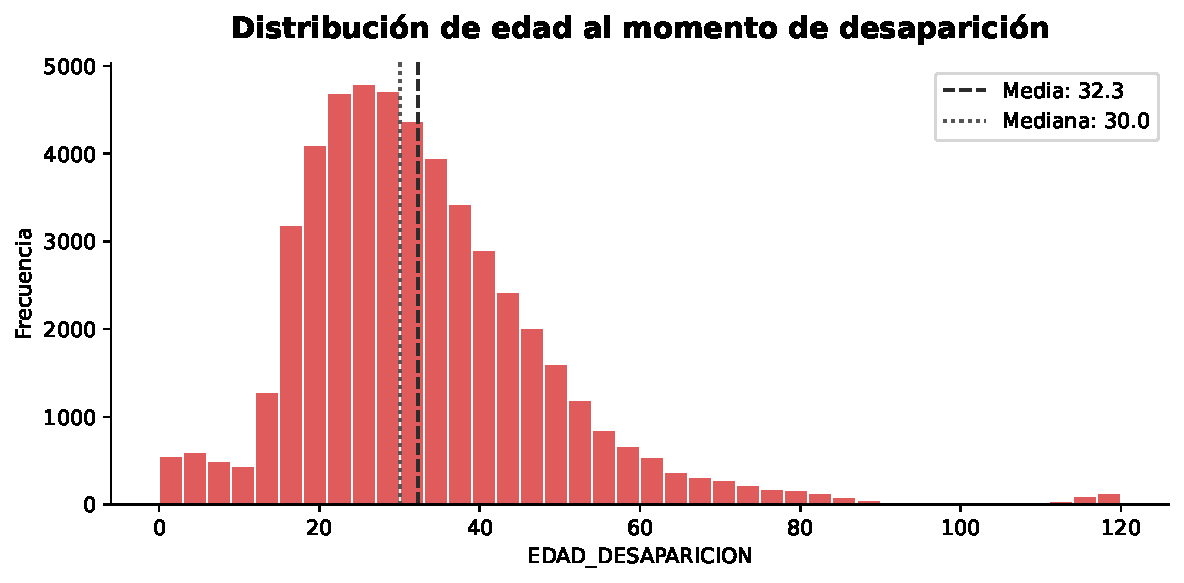
\includegraphics[keepaspectratio]{index_files/figure-pdf/cell-11-output-1.pdf}}

\textsubscript{Source:
\href{https://Rou-uu.github.io/pruebaQuarto/index.qmd.html}{Article
Notebook}}

Esto es claramente un error en el registro de los datos (a menos que
haya personas de 1830 y -13 años), y queremos ver cuantos de estos hay.
Asumiremos que una persona a lo más puede vivir 130 años actualmente,
por lo que veremos cuantas personas hay fuera de ese rango. Podemos ver
que la cantidad no es tanta, sin embargo, cuando reducimos el rango a
100 años como máximo, la cantidad de personas se cuatriplica. Esto
podría significar que efectivamente hay \textasciitilde400 personas que
desaparecieron con más de 100 años, pero también podría significar un
error de dedo al teclear las fechas.

\textsubscript{Source:
\href{https://Rou-uu.github.io/pruebaQuarto/index.qmd.html}{Article
Notebook}}

\begin{verbatim}
Registros fuera del rango [0, 130]: 0
Porcentaje del total: 0.0
\end{verbatim}

\pandocbounded{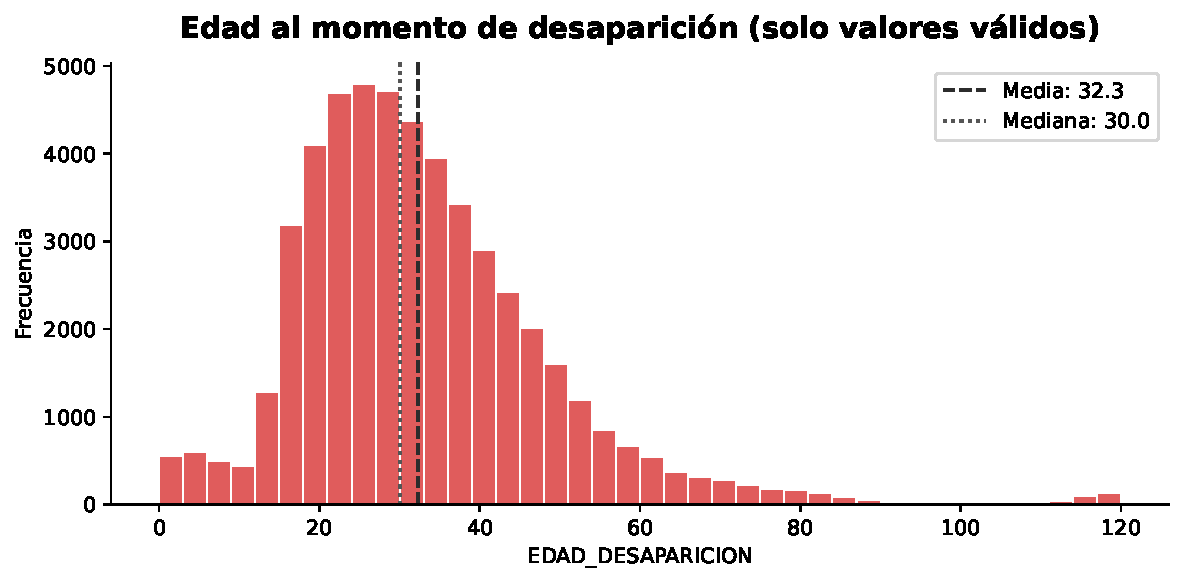
\includegraphics[keepaspectratio]{index_files/figure-pdf/cell-12-output-2.pdf}}

\textsubscript{Source:
\href{https://Rou-uu.github.io/pruebaQuarto/index.qmd.html}{Article
Notebook}}

\subsubsection{SEXO}\label{sexo}

Ahora, calcularemos la moda del sexo de las personas desaparecidas.
Antes de cualqueir cosa, cuando calculamos la moda sobre el dataset
original, la moda es CONFIDENCIAL, por lo que el calculo lo haremos
sobre el dataset ``limpio''

\textsubscript{Source:
\href{https://Rou-uu.github.io/pruebaQuarto/index.qmd.html}{Article
Notebook}}

\begin{verbatim}
0    HOMBRE
Name: SEXO, dtype: str
\end{verbatim}

\textsubscript{Source:
\href{https://Rou-uu.github.io/pruebaQuarto/index.qmd.html}{Article
Notebook}}

La mayor cantidad de personas desaparecidas son hombres. Ahora, si
queremos tratar de ver más allá de esto, no podemos descartar la
posibilidad que dentro de los registros, se mantenga como CONFIDENCIAL
todos aquellos casos que se catalogen como posible secuetro por género
(similar al delito de feminicidio), y que por lo tanto la moda se vea
afectada por esto.

Algunos análisis que podríamos llevar acabo sería ver cual es la moda
por estado, y buscar si por ejemplo, en algún estado en paricular donde
la moda sea mujer, si hay algún problema relacionado al trato de
personas y particularmente mujeres, o en algún estado con moda hombres,
haya problemas por reclutamiento forzado del crimen organizado.

\subsubsection{ESTATUS\_VICTIMA}\label{estatus_victima}

Haremos exactamente el mismo procedimiento que realizamos para el sexo
del dataset

\textsubscript{Source:
\href{https://Rou-uu.github.io/pruebaQuarto/index.qmd.html}{Article
Notebook}}

\begin{verbatim}
0    DESAPARECIDA
Name: ESTATUS_VICTIMA, dtype: str
\end{verbatim}

\textsubscript{Source:
\href{https://Rou-uu.github.io/pruebaQuarto/index.qmd.html}{Article
Notebook}}

En este caso, tampoco hay mucho que se pueda explicar. Simplemente la
mayoría de las personas desaparecidas siguen desaparecidas al día de hoy
(el dataset)

\subsubsection{ENTIDAD}\label{entidad}

Vamos a calcular la moda de la entidad con más desapariciones.

\textsubscript{Source:
\href{https://Rou-uu.github.io/pruebaQuarto/index.qmd.html}{Article
Notebook}}

\begin{verbatim}
0    JALISCO
Name: ENTIDAD, dtype: str
\end{verbatim}

\textsubscript{Source:
\href{https://Rou-uu.github.io/pruebaQuarto/index.qmd.html}{Article
Notebook}}

Esta medida es particular. Podemos ver que si nos guiamos por la
cantidad de elementos ``eliminados'' por ser confidenciales/nulos, la
moda debería de ser el Estado de México, pues es el estado que tiene el
mayor número de información disponible. Sin embargo, esta es una de las
medidas que no se ve afectada por la falta de información. Todas las
filas tienen un valor en ENTIDAD válido, por lo que aunque no sepamos
acerca de la información precisa del casos de desaparición, al menos
tenemos conocimiento del estado del que se reporto, por lo que no
perdemos información por confidencialidad.

\subsubsection{MUNICIPIO}\label{municipio}

Para esta medida sacaremos la moda, sin embargo, esta medida puede no
resultar de gran utilidad al realizar el analisis en todo el dataset en
lugar de hacerlo por entidad, debido a que podría sucede que por
ejemplo, el municipio donde más haya desapariciones sea en un estado con
la menor cantidad de desapariciones, lo cual a su vez podría suceder
debido a que ENTIDAD no tiene información confidencial, pero los
MUNICIPIO si, por lo que la relación que podríamos buscar se podría ver
sesgada por eso.

\textsubscript{Source:
\href{https://Rou-uu.github.io/pruebaQuarto/index.qmd.html}{Article
Notebook}}

\begin{verbatim}
0    SE DESCONOCE
Name: MUNICIPIO, dtype: str
\end{verbatim}

\textsubscript{Source:
\href{https://Rou-uu.github.io/pruebaQuarto/index.qmd.html}{Article
Notebook}}

Aún así, la moda resultó ser municipio desconocido.

\subsubsection{FECHA\_DESAPARICION}\label{fecha_desaparicion}

Para la fecha de desaparicion sacaremos la moda y la mediana. Además,
podemos gráficar la cantidad de desapariciones por año para ver una
tendencia respecto al tiempo que ha pasado entre la primera desaparicion
y la última.

\textsubscript{Source:
\href{https://Rou-uu.github.io/pruebaQuarto/index.qmd.html}{Article
Notebook}}

\begin{verbatim}
Mediana de fecha de desaparición: 2018-09-21
Moda de fecha de desaparición: 1974-01-01
\end{verbatim}

\textsubscript{Source:
\href{https://Rou-uu.github.io/pruebaQuarto/index.qmd.html}{Article
Notebook}}

De ver la mediana, nos damos cuenta que al menos 50\% de las
desapariciones registradas en este dataset han sido registradas a partir
del 2018, a pesar de que el día con más desapariciones fue en 1974. Esto
podría ser por la precision con la que estamos calculando la moda. En la
gráfica de abajo vemos que el año con más desapariciones fue 2024
(aprox), por lo que si hiciermos una moda por año, el resultado sería
distinto. Hacer la moda por día no resulta muy útil, y además puede
llevar a malinterpretar los resultados. Si no sacaramos medaiana, y
solamente nos guiaramos por la moda del día, pensaríamos que la
inseguridad es menor acutalmente, a pesar de que la gráfica de abajo
muestra que la tendencía de desapariciones va en aumento.

\textsubscript{Source:
\href{https://Rou-uu.github.io/pruebaQuarto/index.qmd.html}{Article
Notebook}}

\pandocbounded{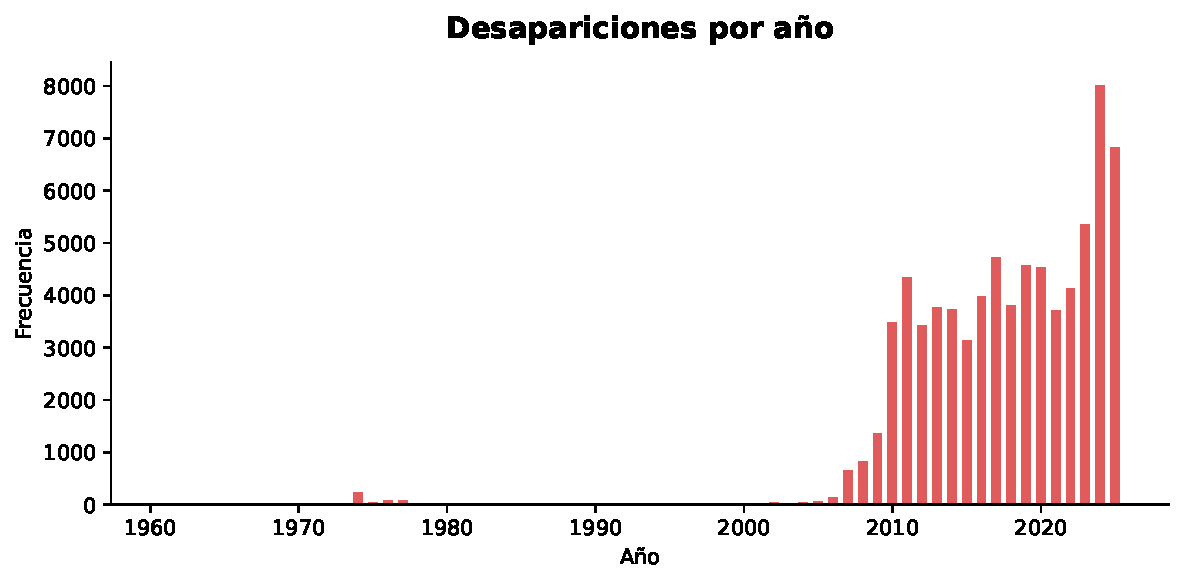
\includegraphics[keepaspectratio]{index_files/figure-pdf/cell-18-output-1.pdf}}

\textsubscript{Source:
\href{https://Rou-uu.github.io/pruebaQuarto/index.qmd.html}{Article
Notebook}}

\subsection{Analisis de variabilidad}\label{analisis-de-variabilidad}

Las medidas que estaremos utilizando serán las siguientes: \textbar{}
Variable \textbar{} Medidas \textbar{}
\textbar---------------------\textbar----------------------------------------------\textbar{}
\textbar{} EDAD\_DESAPARICION \textbar{} Varianza, rango, IQR,
desviación estandar \textbar{} \textbar{} FECHA\_DESAPARICION \textbar{}
Mínimo, máximo, rango \textbar{} \textbar{} FECHA\_REGISTRO \textbar{}
Mínimo, máximo, rango \textbar{}

Como no tenemos variables númericas además de la edad, hacer un análisis
de variabilidad de los datos resulta complicado. Sin embargo, podemos
realizar un buen analisis sobre la edad de desaparición.

\subsubsection{EDAD\_DESAPARICION}\label{edad_desaparicion-1}

Para la edad de desaparición, sacaremos la varianza, el rango, el IQR, y
la desviación estandar. Primero lo haremos con el dataset con el rango
sin ajustar, y luego lo haremos con el rango ajustado. Debido a que los
valores son extremos, deberíamos de ver un cambio en la mayoría de las
medidas.

\textsubscript{Source:
\href{https://Rou-uu.github.io/pruebaQuarto/index.qmd.html}{Article
Notebook}}

\begin{verbatim}
Varianza: 249.74
Desviación estándar: 15.80
Rango: 120.00
Rango intercuartílico (IQR): 18.00
\end{verbatim}

\textsubscript{Source:
\href{https://Rou-uu.github.io/pruebaQuarto/index.qmd.html}{Article
Notebook}}

\begin{verbatim}
Varianza: 249.74
Desviación estándar: 15.80
Rango: 120.00
Rango intercuartílico (IQR): 18.00
\end{verbatim}

\textsubscript{Source:
\href{https://Rou-uu.github.io/pruebaQuarto/index.qmd.html}{Article
Notebook}}

Podemos observar que si hubo un cambio medianamente grande. Ver un
cambio de aproximadamente 5 años en la desviación estandar significa que
podemos ajustar de mejor forma la cantidad de casos y buscar una
generalidad. Como la desviación es de 15.81 años, y el promedio es de
\textasciitilde32 años, significa que la mayoría de los casos de
desapariciones estan en el rango de {[}17 - 45{]} años de edad. Eso
significa que los dos grupos más afectados por las desapariciones son
los jovenes y los adultos, pero eso forma gran parte de la población,
por lo que no podríamos decir que este desapareciendo un cierto perfil
de edad.

\subsubsection{FECHA\_DESAPARICION}\label{fecha_desaparicion-1}

Para la fecha de desaparición podemos sacar un rango de valores, pero
eso ya lo calculamos e hicimos un breve análisis en la sección anterior,
por lo que aquí no lo pondremos

\subsubsection{FECHA\_REGISTRO}\label{fecha_registro}

Sacaremos el rango de valores de las fechas de registro de incidentes.
Recordemos que anteriormente calculamos las edades al momento de la
desaparición usando la de nacimiento y registro. Obtuvimos valores que
no tenían sentido, y vimos que en muchos casos esos valores eran por
fechas de nacimeinto mal escritas. Igualmente, podría ser que haya
fechas de registro que este causando un cálculo erroneo de la edad de
las personas, por lo que eso lo podremos ver en el rango.

\textsubscript{Source:
\href{https://Rou-uu.github.io/pruebaQuarto/index.qmd.html}{Article
Notebook}}

\begin{verbatim}
Fecha mínima de registro: 1961-05-08
Fecha máxima de registro: 2025-10-01
Rango de fechas de registro: 64.44383561643835 años
\end{verbatim}

\textsubscript{Source:
\href{https://Rou-uu.github.io/pruebaQuarto/index.qmd.html}{Article
Notebook}}

En este caso no vemos valores anormales, lo que se puede deber a que el
registro de las fechas se hace de forma automática en el sistema,
evitando errores como los de las fechas de nacimiento. Además, vemos que
el dataset cubre las desapariciones de aproximadamente 65 años.

\subsection{Analisis de
heterogeneidad}\label{analisis-de-heterogeneidad}

Buscamos cuantificar qué tan ``mezclados'' o diversos son los datos
dentro de nuestras variables categóricas nominales. Las medidas que
estaremos utilizando serán las siguientes:

{\def\LTcaptype{none} % do not increment counter
\begin{longtable}[]{@{}ll@{}}
\toprule\noalign{}
Variable & Medidas \\
\midrule\noalign{}
\endhead
\bottomrule\noalign{}
\endlastfoot
SEXO & Entropía de Shannon, índice de Simpson \\
ESTATUS\_VICTIMA & Entropía de Shannon \\
ENTIDAD & Entropía de Shannon \\
MUNICIPIO & Entropía de Shannon \\
ORIGEN\_REPORTE & Entropía de Shannon \\
\end{longtable}
}

\textsubscript{Source:
\href{https://Rou-uu.github.io/pruebaQuarto/index.qmd.html}{Article
Notebook}}

\textsubscript{Source:
\href{https://Rou-uu.github.io/pruebaQuarto/index.qmd.html}{Article
Notebook}}

\subsubsection{SEXO}\label{sexo-1}

\textsubscript{Source:
\href{https://Rou-uu.github.io/pruebaQuarto/index.qmd.html}{Article
Notebook}}

\begin{verbatim}
ANÁLISIS DE DIVERSIDAD: SEXO
--- Análisis de Heterogeneidad: SEXO ---
Entropía de Shannon: 0.8202 bits
Índice de Simpson (Dominancia): 0.6365
Diversidad de Simpson (1-D): 0.3635
\end{verbatim}

\pandocbounded{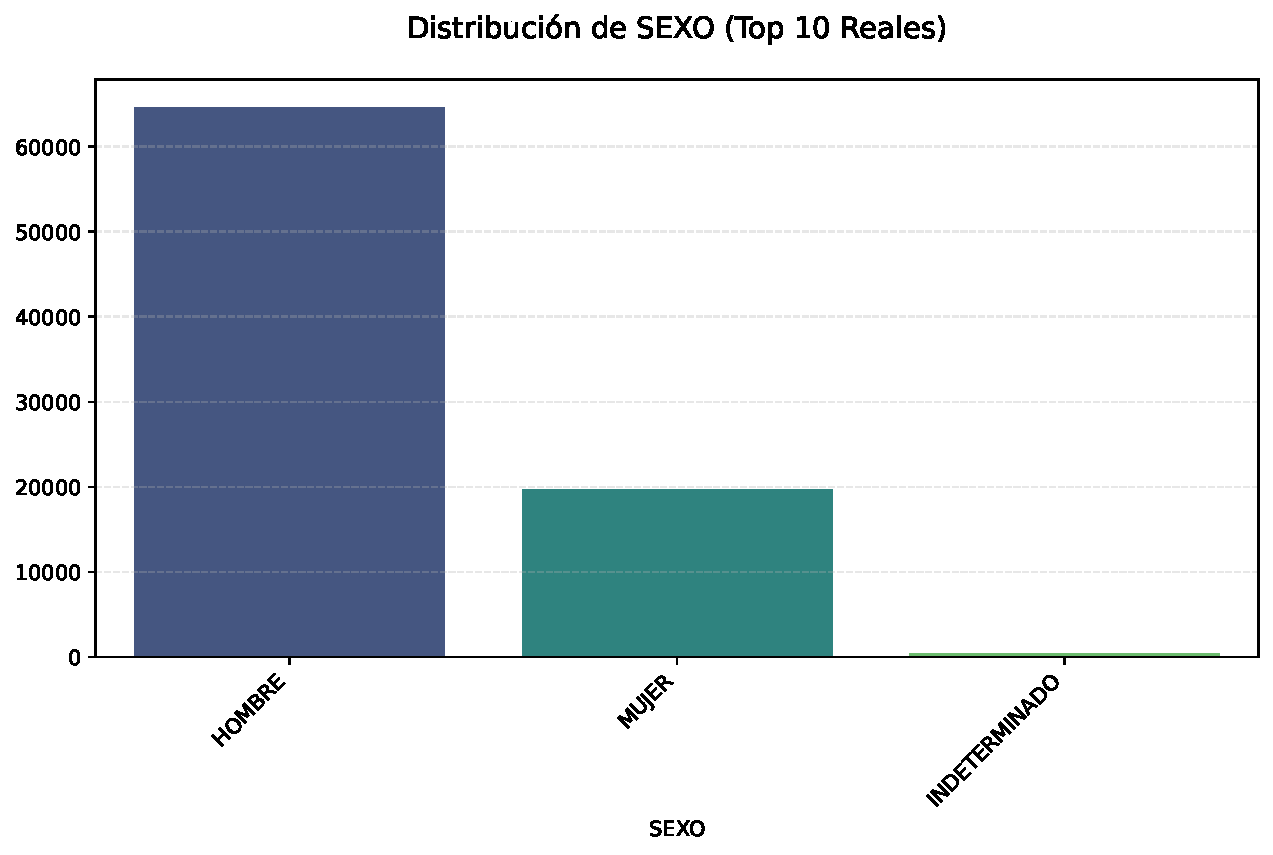
\includegraphics[keepaspectratio]{index_files/figure-pdf/cell-23-output-2.pdf}}

\textsubscript{Source:
\href{https://Rou-uu.github.io/pruebaQuarto/index.qmd.html}{Article
Notebook}}

Aunque hay víctimas de distintos géneros, los datos no están repartidos
de forma equilibrada. Hay una mayoría tan clara de hombres que las
estadísticas se inclinan fuertemente hacia ellos, dejando claro que no
es un fenómeno que afecte de forma equitativa a toda la población.

\subsubsection{ESTATUS\_VICTIMA}\label{estatus_victima-1}

\textsubscript{Source:
\href{https://Rou-uu.github.io/pruebaQuarto/index.qmd.html}{Article
Notebook}}

\begin{verbatim}
ANÁLISIS DE DIVERSIDAD: ESTATUS_VICTIMA
--- Análisis de Heterogeneidad: ESTATUS_VICTIMA ---
Entropía de Shannon: 0.3167 bits
Índice de Simpson (Dominancia): 0.8919
Diversidad de Simpson (1-D): 0.1081
\end{verbatim}

\pandocbounded{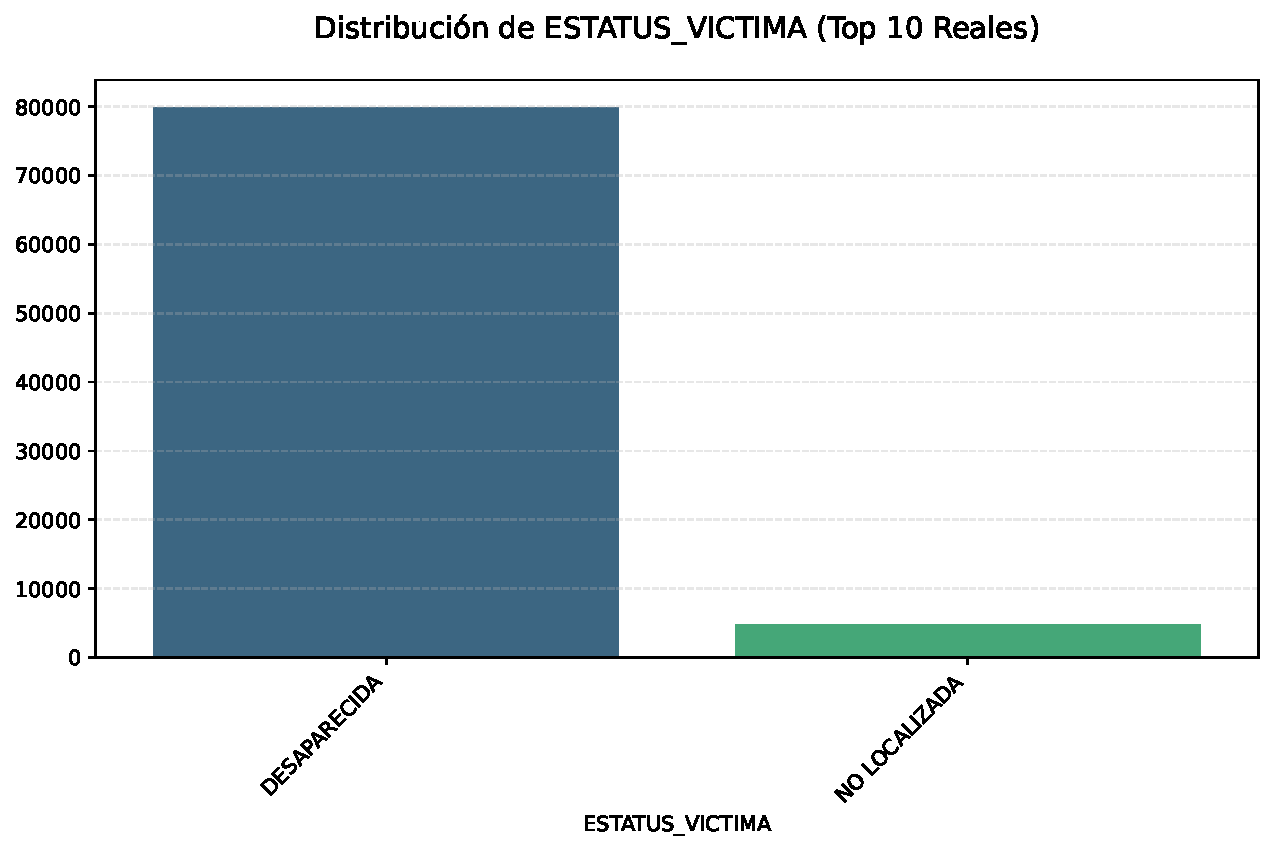
\includegraphics[keepaspectratio]{index_files/figure-pdf/cell-24-output-2.pdf}}

\textsubscript{Source:
\href{https://Rou-uu.github.io/pruebaQuarto/index.qmd.html}{Article
Notebook}}

Al haber un índice de Simpson alto, significa que hay una categoría que
``domina'' a todas las demás. La inmensa mayoría de las personas en la
lista siguen en calidad de desaparecidas. No hay un equilibrio entre
personas encontradas y no encontradas; el dataset está ``estancado'' en
una sola situación.

\subsubsection{ENTIDAD}\label{entidad-1}

\textsubscript{Source:
\href{https://Rou-uu.github.io/pruebaQuarto/index.qmd.html}{Article
Notebook}}

\begin{verbatim}
ANÁLISIS DE DIVERSIDAD: ENTIDAD FEDERATIVA
--- Análisis de Heterogeneidad: ENTIDAD ---
Entropía de Shannon: 4.4605 bits
Índice de Simpson (Dominancia): 0.0580
Diversidad de Simpson (1-D): 0.9420
\end{verbatim}

\pandocbounded{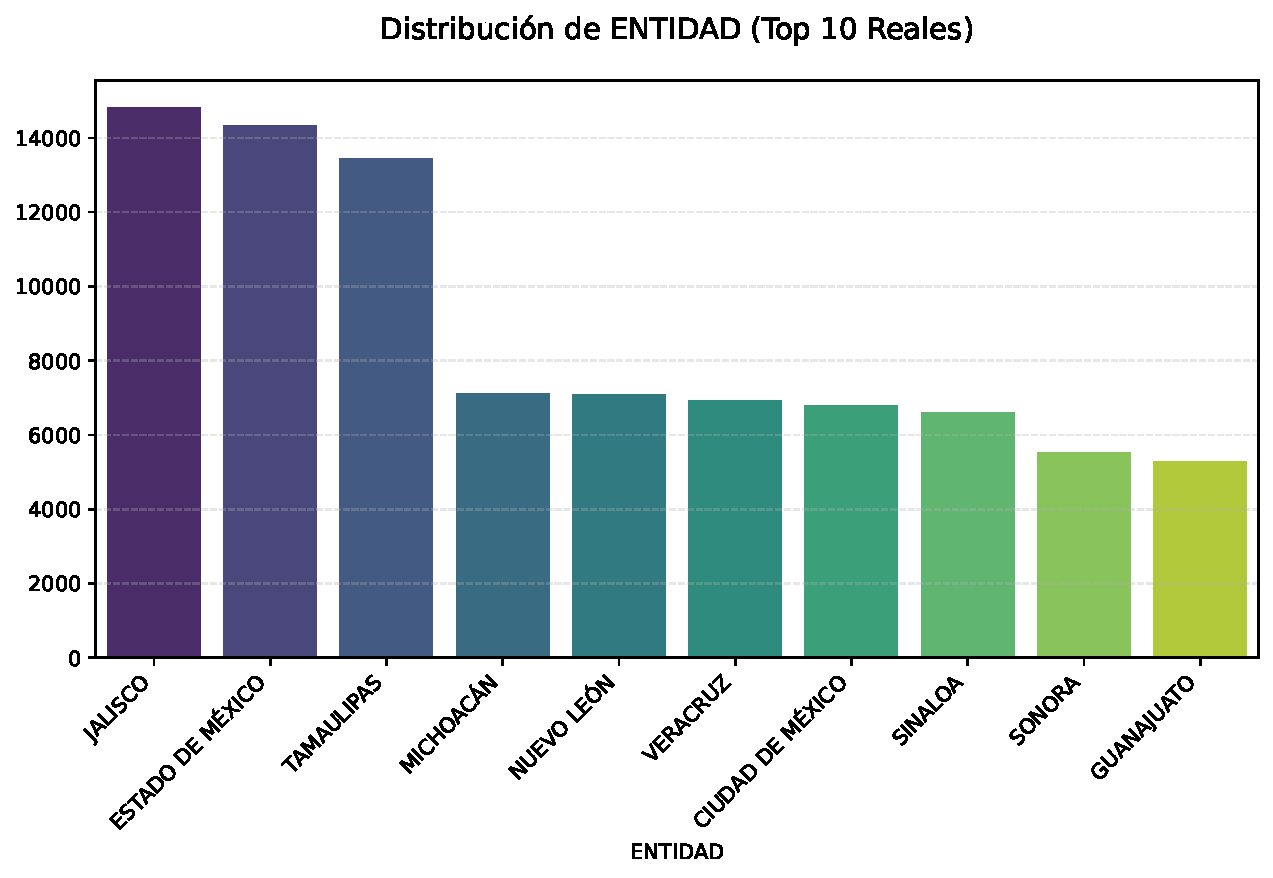
\includegraphics[keepaspectratio]{index_files/figure-pdf/cell-25-output-2.pdf}}

\textsubscript{Source:
\href{https://Rou-uu.github.io/pruebaQuarto/index.qmd.html}{Article
Notebook}}

La variable ENTIDAD presenta la mayor entropía de Shannon del dataset.
Esto confirma que las desapariciones son un fenómeno generalizado. No es
algo que le pase a ``un solo estado'', sino que es un problema que
afecta a múltiples regiones de México casi por igual, lo que lo hace
mucho más difícil de controlar.

\subsubsection{MUNICIPIO}\label{municipio-1}

\textsubscript{Source:
\href{https://Rou-uu.github.io/pruebaQuarto/index.qmd.html}{Article
Notebook}}

\begin{verbatim}
ANÁLISIS DE DIVERSIDAD: MUNICIPIO
--- Análisis de Heterogeneidad: MUNICIPIO ---
Entropía de Shannon: 8.2014 bits
Índice de Simpson (Dominancia): 0.0101
Diversidad de Simpson (1-D): 0.9899
\end{verbatim}

\pandocbounded{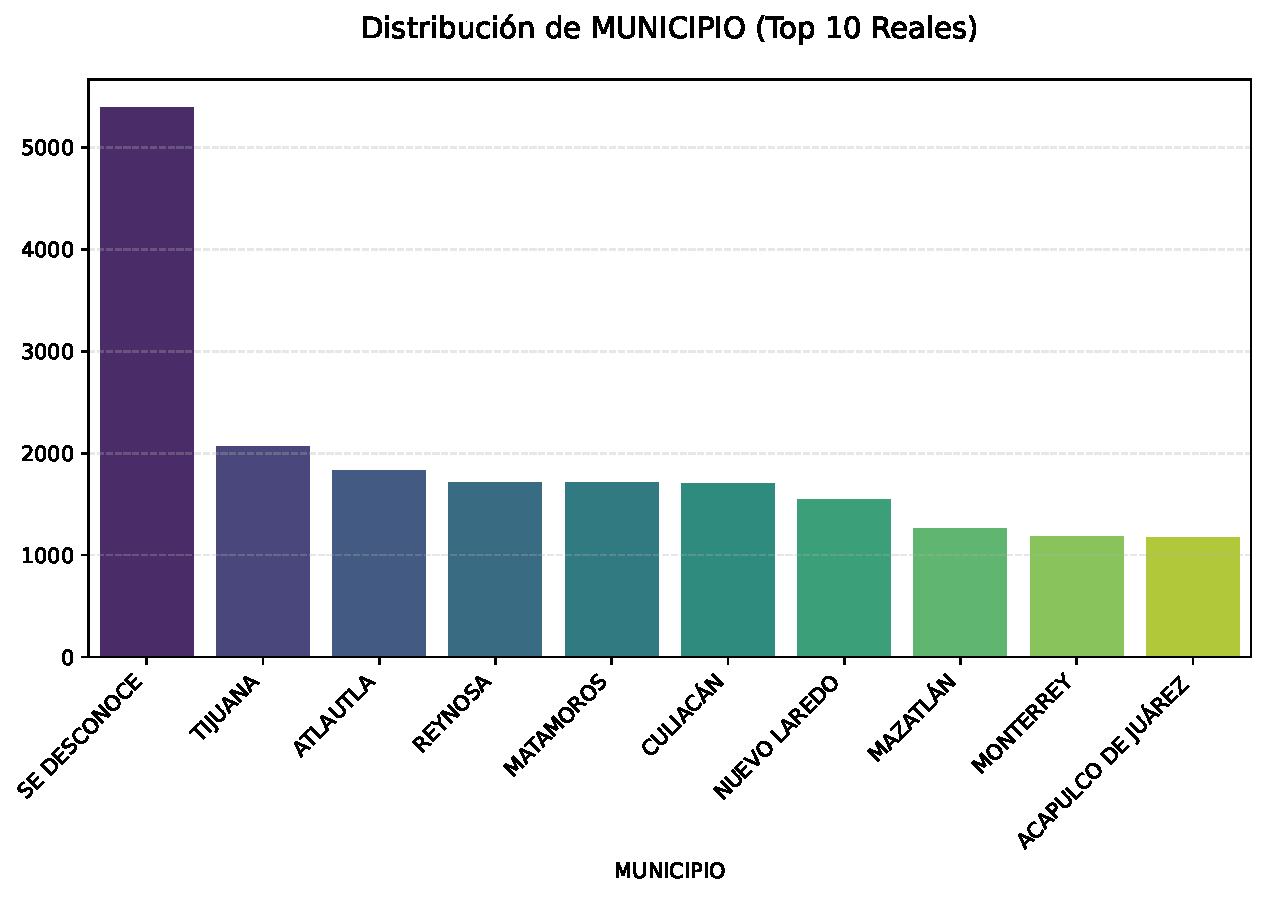
\includegraphics[keepaspectratio]{index_files/figure-pdf/cell-26-output-2.pdf}}

\textsubscript{Source:
\href{https://Rou-uu.github.io/pruebaQuarto/index.qmd.html}{Article
Notebook}}

A nivel municipal, el problema es tan variado que es difícil predecir
dónde ocurrirá un caso (entropía alta). Sin embargo, hay ciudades
específicas donde el fenómeno deja de estar repartido y se vuelve mucho
más frecuente, lo que las convierte en zonas de alto riesgo local.
También destaca que en muchos casos no se tiene el dato exacto del
lugar, lo que dificulta el análisis preciso.

\subsubsection{ORIGEN\_REPORTE}\label{origen_reporte}

\textsubscript{Source:
\href{https://Rou-uu.github.io/pruebaQuarto/index.qmd.html}{Article
Notebook}}

\begin{verbatim}
ANÁLISIS DE DIVERSIDAD: ORIGEN_REPORTE
--- Análisis de Heterogeneidad: ORIGEN_REPORTE ---
Entropía de Shannon: 5.1607 bits
Índice de Simpson (Dominancia): 0.0384
Diversidad de Simpson (1-D): 0.9616
\end{verbatim}

\pandocbounded{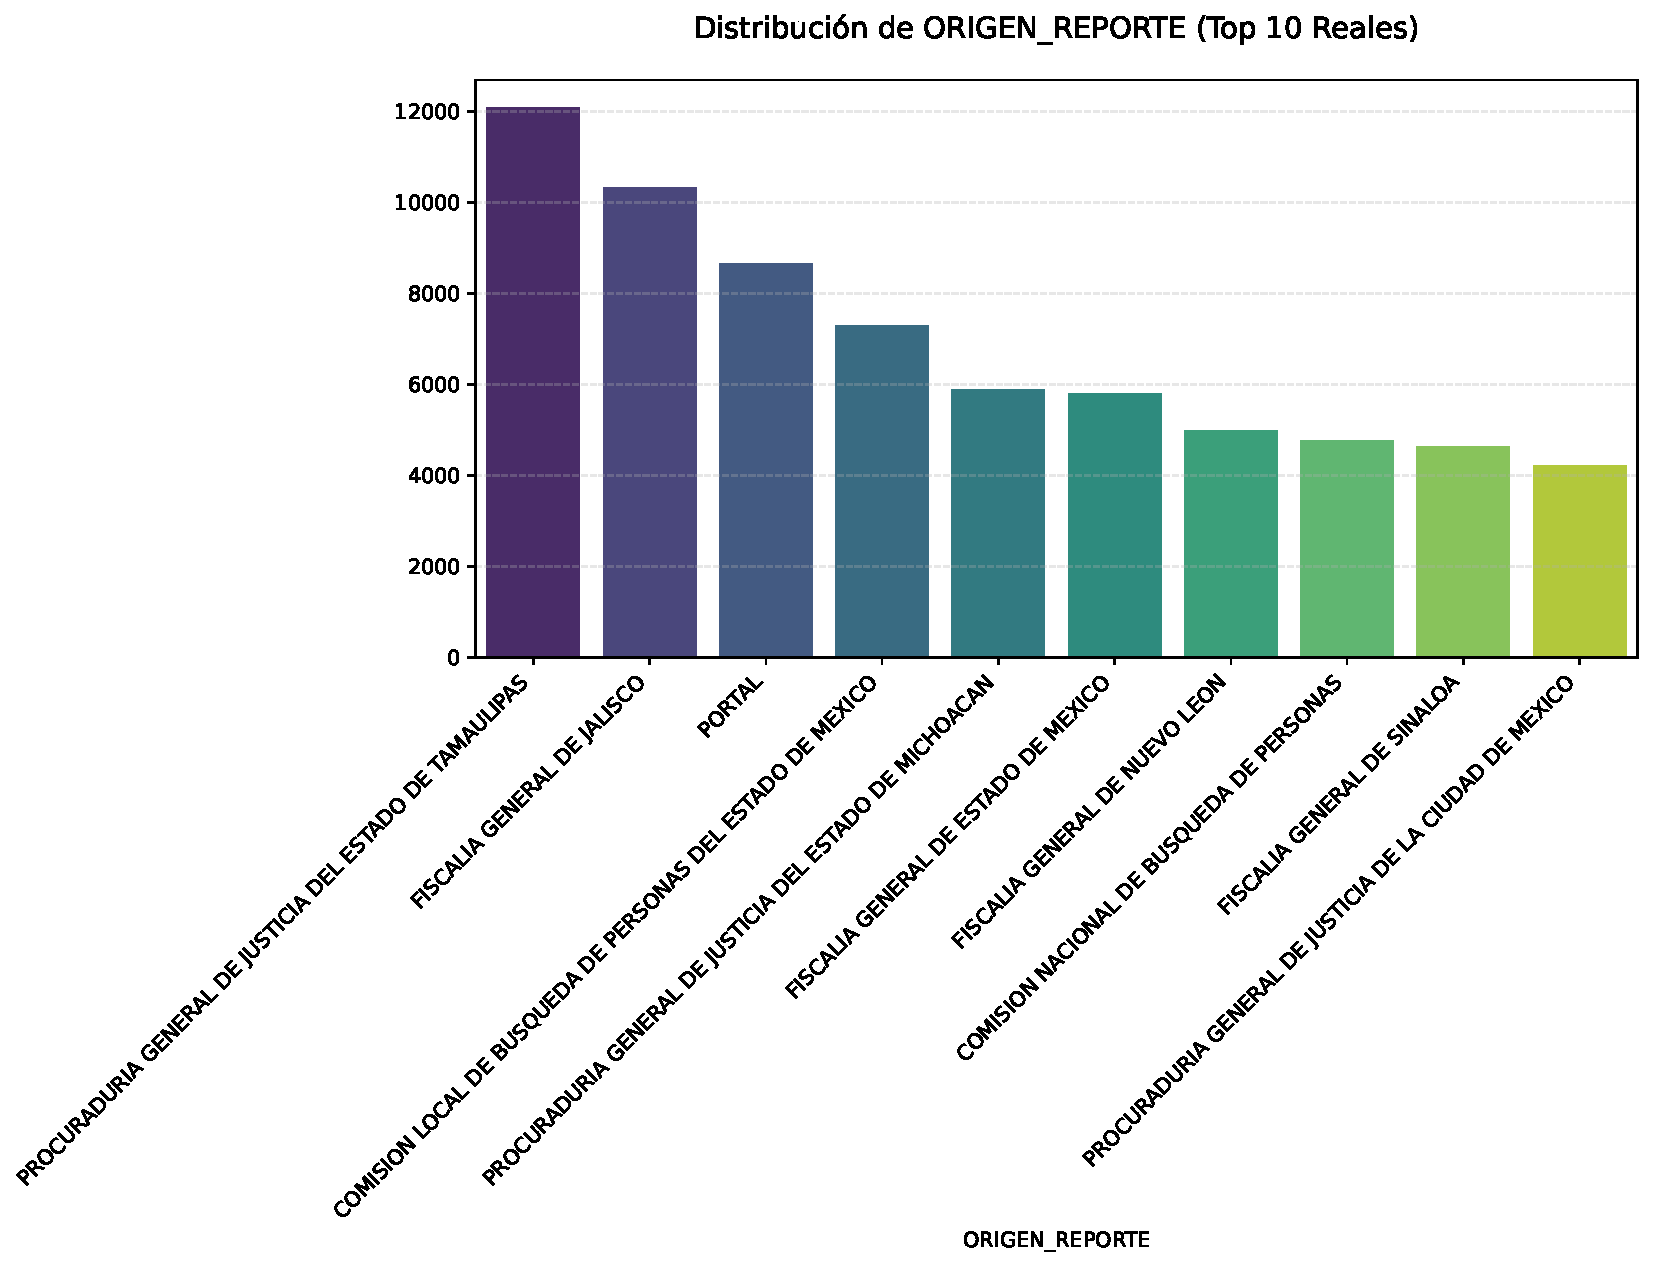
\includegraphics[keepaspectratio]{index_files/figure-pdf/cell-27-output-2.pdf}}

\textsubscript{Source:
\href{https://Rou-uu.github.io/pruebaQuarto/index.qmd.html}{Article
Notebook}}

Analizar el Origen del Reporte es como revisar la salud de nuestras
fuentes. Si los datos vienen de muchos lugares distintos, nuestro
análisis es más confiable y democrático. Si vienen de uno solo, estamos
viendo la realidad a través de un solo lente, lo que podría ocultar lo
que otras instituciones están reportando.

\subsection{Analisis de
concentración}\label{analisis-de-concentraciuxf3n}

Las medidas que estaremos sacando son:

{\def\LTcaptype{none} % do not increment counter
\begin{longtable}[]{@{}ll@{}}
\toprule\noalign{}
Variable & Medidas \\
\midrule\noalign{}
\endhead
\bottomrule\noalign{}
\endlastfoot
SEXO & Freciencia relativa a la moda \\
ENTIDAD & HHI \\
MUNICIPIO & HHI \\
EDAD\_DESAPARICION & Indice de Gini y Curva de Lorenz \\
\end{longtable}
}

\subsubsection{SEXO}\label{sexo-2}

\textsubscript{Source:
\href{https://Rou-uu.github.io/pruebaQuarto/index.qmd.html}{Article
Notebook}}

\begin{verbatim}
--- Concentración en SEXO ---
Moda: HOMBRE
Frecuencia relativa de la moda: 0.7631 (76.31%)
\end{verbatim}

\textsubscript{Source:
\href{https://Rou-uu.github.io/pruebaQuarto/index.qmd.html}{Article
Notebook}}

Al calcular la frecuencia relativa de la moda, observamos que una sola
categoría absorbe la gran mayoría de los registros.

\subsubsection{Concentración Geográfica (HHI de Entidad y
Municipio)}\label{concentraciuxf3n-geogruxe1fica-hhi-de-entidad-y-municipio}

\textsubscript{Source:
\href{https://Rou-uu.github.io/pruebaQuarto/index.qmd.html}{Article
Notebook}}

\begin{verbatim}
Índice HHI (Entidad Federativa): 579.85
Índice HHI (Municipio): 100.74
\end{verbatim}

\textsubscript{Source:
\href{https://Rou-uu.github.io/pruebaQuarto/index.qmd.html}{Article
Notebook}}

El Índice HHI nos dice si el peligro está ``amontonado'' en unos pocos
puntos del mapa o si está repartido por todos lados. Un valor alto en
los Estados confirmaría que solo un puñado de entidades concentran la
gran mayoría de los casos, convirtiéndose en los ``dueños'' del
problema. En cambio, en los Municipios, aunque el índice suele ser bajo
porque hay miles de localidades, el HHI nos ayuda a detectar si ciudades
específicas están absorbiendo un nivel de riesgo desproporcionado
comparado con el resto del país.

\subsubsection{EDAD\_DESAPARICION}\label{edad_desaparicion-2}

\textsubscript{Source:
\href{https://Rou-uu.github.io/pruebaQuarto/index.qmd.html}{Article
Notebook}}

\pandocbounded{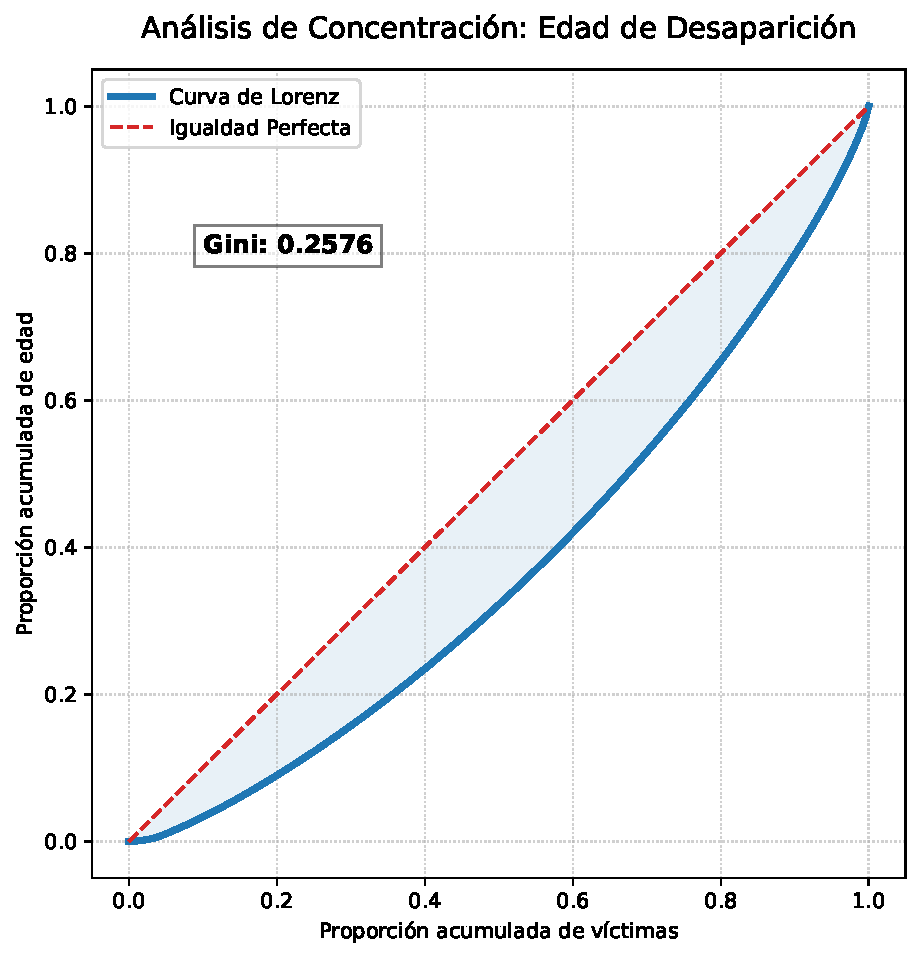
\includegraphics[keepaspectratio]{index_files/figure-pdf/cell-30-output-1.pdf}}

\textsubscript{Source:
\href{https://Rou-uu.github.io/pruebaQuarto/index.qmd.html}{Article
Notebook}}

La Curva de Lorenz y el Coeficiente de Gini demuestran que las
desapariciones no ocurren en todas las edades. Al observar una
desviación clara respecto a la igualdad, confirmamos que el riesgo se
concentra en sectores específicos (principalmente jóvenes). Esto nos
permite pasar de un análisis general a uno enfocado, identificando
perfiles de vulnerabilidad que son fundamentales para diseñar
estrategias de prevención y búsqueda criminalística.

\textsubscript{Source:
\href{https://Rou-uu.github.io/pruebaQuarto/index.qmd.html}{Article
Notebook}}




\end{document}
